%%p01
$(x+4)(x-7)$
%%a01
\begin{enum}
	* $x^2-28$
	* $x^3-4x+26$
	* $x^2+3x-14$
	* $x^2-3x-28$
\end{enum}
%%r01
$x^2-3x-28$
%%p02
$(2x-1)\cdot(3-x)$
%%a02
\begin{enum}
	* $6x-3x^2-2$
	* $7x^2+2x-3$
	* $5x+3x^2-2$
	* $7x-2x^2-3$
\end{enum}
%%r02
$7x-2x^2-3$
%%p03
$(x-3y)(x+2y)$
%%a03
\begin{enum}
	* $x^2-xy-6y^2$
	* $-x-xy+6x^2y$
	* $2x^2+xy+9y$
	* $4xy+xy-6y$
\end{enum}
%%r03
$x^2-xy-6y^2$
%%p04
$(2x+3)\cdot(7x-5)$
%%a04
\begin{enum}
	* $14x^2+11x-15$
	* $-14x^2+11-15$
	* $6x^2-21+16$
	* $21x^2+11x-16$
\end{enum}
%%r04
$14x^2+11x-15$
%%p05
$\left(x^7\div x^5\right)\cdot\left(x^3\div x\right)$
%%a05
\begin{enum}
	* $x^2$
	* $x^4$
	* $x^6$
	* $x^3$
\end{enum}
%%r05
$x^4$
%%p06
$(2x-3y)^2$
%%a06
\begin{enum}
	* $3x^2+6xy-9y^2$
	* $4x^2-12xy+9y^2$
	* $4x^2+12xy-9y^2$
	* $2x^3-8xy-3y^2$
\end{enum}
%%r06
$4x^2-12xy+9y^2$
%%p07
$\left(18x^3y^2z^5\right)\cdot\left(6x^3yz^2\right)$
%%a07
\begin{enum}
	* $120x^3y^5z$
	* $-180x^3yz^2$
	* $108x^6y^3z^7$
	* $-120x^3yz$
\end{enum}
%%r07
$108x^6y^3z^7$
%%p08
$\dfrac{6x^3-3x^2+9x-4}{3}$
%%a08
\begin{enum}
	* $x^7-x^4+3x-\dfrac{4}{5}$
	* $2x^4-x^9+4x-\dfrac{7}{6}$
	* $x^3-x^6+9x-\dfrac{43}{3}$
	* $2x^3-x^2+3x-\dfrac{4}{3}$
\end{enum}
%%r08
$2x^3-x^2+3x-\dfrac{4}{3}$
%%p09
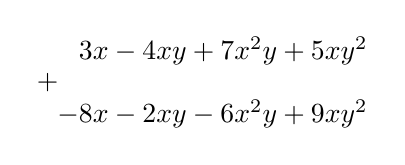
\begin{tikzpicture}
	\node[right] at (0,.4) {$\phantom{-}3x-4xy+7x^2y+5xy^2$};
	\node[right] at (0,-.4) {$-8x-2xy-6x^2y+9xy^2$};
	\node at (0,0) {$+$};
\end{tikzpicture}
%%a09
\begin{enum}
	* $-5+7xy-x^2y-4xy^2$
	* $5+7yx-x^3y-4xy^4$
	* $-5x-6xy+x^2y+14xy^2$
	* N.A.
\end{enum}
%%r09
$-5x-6xy+x^2y+14xy^2$
%%p10
$2\left(x^2+x\right)-9\left(x^2-2x\right)$
%%a10
\begin{enum}
	* $-18x-7x^2$
	* $-10x$
	* $7x^2-10x$
	* $-7x^2+20x$
\end{enum}
%%r10
$-7x^2+20x$
%%p11
$2x\left(14y^4+8x^2-4x^9+2^8\right)$
%%a11
\begin{enum}
	* $28xy^4-8x^{10}+16x^3+512x$
	* $28xy^4-16x^3+8x^{10}+256x$
	* $14xy^4+16xy-8x^2+256x$
	* $28xy^4-16x^3-8x^{10}+512x$
\end{enum}
%%r11
$28xy^4-8x^{10}+16x^3+512x$
%%p12
$\GR(x)+\GR(y)$ de $2y^4+8x^9+29a^2$
%%a12
\begin{enum}
	* $12$
	* $9$
	* $10$
	* $13$
\end{enum}
%%r12
$13$
%%p13
$\GA(x,y,z)+\GR(y)$ de \\
$64x^{12}y^8z^9+32y^{15}+x^4$
%%a13
\begin{enum}
	* $44$
	* $42$
	* $41$
	* $40$
\end{enum}
%%r13
$44$
%%p14
Calcular ``$a$'' si el $\GR(x)=4$; en: \\
$P_{(x,y)}=2x^{a+3}y^5+7x^ay^8$
%%a14
\begin{task}
	* $\dfrac{1}{5}$
	* $1$
	* $\dfrac{2}{6}$
	* $\dfrac{1}{2}$
\end{task}
%%r14
$1$
%%p15
\begin{tabular}{c}
	Calcula $a+b$, si son términos semejantes: \\
	$\begin{aligned}
		T_1&=2x^{3a-6}y^{\frac{b-1}{5}} \\
		T_2&=\dfrac{-\sqrt{3}}{5}x^3y^2
	\end{aligned}$
\end{tabular}
%%a15
\begin{enum}
	* $12$
	* $14$
	* $15$
	* $13$
\end{enum}
%%r15
$14$
